\documentclass[a4paper]{article}
\usepackage{amsmath, amssymb, bm}
\usepackage[margin=1in]{geometry}
\usepackage{graphicx}
\begin{document}
	\begin{titlepage}
		\centering
		{\huge \bf Assignment 4\par}
		\vspace{1cm}
		{\Large Computational Intelligence, SS2018\par}
		\vspace{1cm}
		\begin{tabular}{|l|l|l|}
			\hline
			\multicolumn{3}{|c|}{\textbf{Team Members}}   \\ \hline
			Last name & First name & Matriculation Number \\ \hline
			Lee       & Eunseo     & 11739623             \\ \hline
			Shadley   & Alex       & 11739595             \\ \hline
			Lee       & Dayeong    & 11730321             \\ \hline
		\end{tabular}
	\end{titlepage}

\section{Maximum Likelihood Estimation of Model Parameters}
\subsection{Find out which is the anchor with exponentially distributed measurements}

To find out which anchor is with exponentially distributed measurements, I used Kolmogorov-Smirnov test.\newline
The following picture is the KS test statistic with parameter "expon", which is exponential distribution, for each anchor.

\begin{figure}[h]
	\begin{center}
	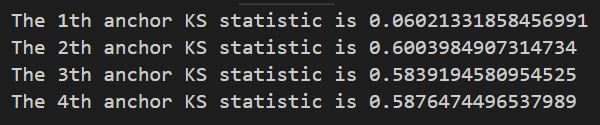
\includegraphics[width=0.5\textwidth]{kstest.jpg}
	\caption{KS test statistic}
	\end{center}
\end{figure}

If KS statistic is close to 0, it means that the dataset is similar with the parameter distribution. \textbf{First anchor} KS statistic is close to 0. Therefore, first anchor follows exponential distribution because above KS test parameter is exponential distribution.

\subsection{Analytically derive the maximum likelihood solution for the exponential distribution}

\subsection{Estimate the parameters of the measurement models}
\subsubsection{Scenario 1: Measurements of all anchors follow the Gaussian model.}
\begin{figure}[h]
	\begin{center}
		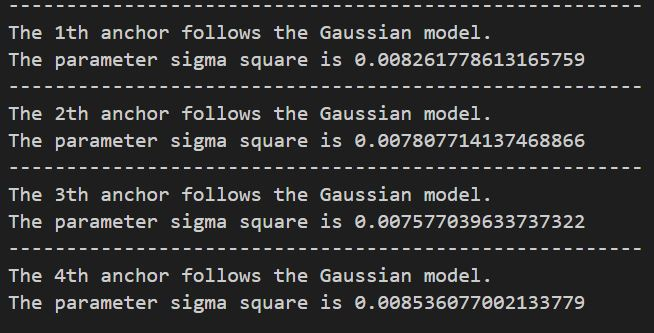
\includegraphics[width=0.5\textwidth]{scenario1param.jpg}
		\caption{Parameters for each anchor}
	\end{center}
\end{figure}
\clearpage
\subsubsection{Scenario 2: Measurements of one anchor follow the Exponential model, the other ones follow the Gaussian model.}
\begin{figure}[h]
	\begin{center}
		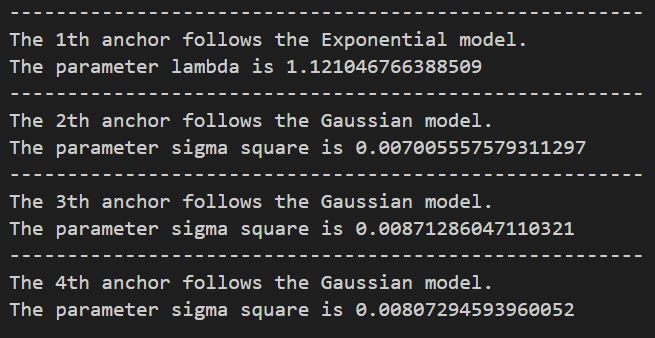
\includegraphics[width=0.5\textwidth]{scenario2param.jpg}
		\caption{Parameters for each anchor}
	\end{center}
\end{figure}

\subsubsection{Measurements of all anchors follow the Exponential model.}
\begin{figure}[h]
	\begin{center}
		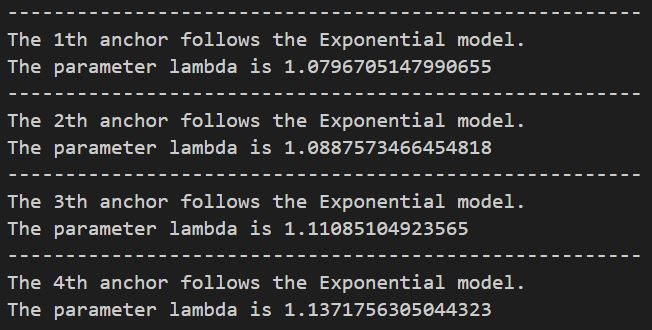
\includegraphics[width=0.5\textwidth]{scenario3param.jpg}
		\caption{Parameters for each anchor}
	\end{center}
\end{figure}

\section{Estimation of the Position}
\subsection{Least-Squares Estimation of the Position}
\subsection{Numerical Maximum-Likelihood Estimation of the Position}

\end{document}